\documentclass[10pt,a4paper]{report}

\usepackage[margin=1in]{geometry}
\usepackage[utf8]{inputenc}
\usepackage{amsmath}
\usepackage{import} 
\usepackage{titlepic} %picture in front
\usepackage{graphicx}
\usepackage{amsfonts}
\usepackage{amssymb}
\usepackage{hyperref} %\usepackage[hidelinks]{hyperref} % use that to remove boxes. 
\usepackage[]{mcode} %for matlab code, uses local package 
\usepackage{tikz}%drawings and diagrams
\usetikzlibrary{calc,patterns,decorations.pathmorphing,decorations.markings}
\usepackage{chngcntr}
\counterwithin*{chapter}{part}
\usepackage{siunitx}%phyisical quantities typesettings
	\usepackage{blkarray}
\usepackage{multirow}
\usepackage{pgfplots} %plots
\usepackage[backend=bibtex]{biblatex}
\addbibresource{biblio.bib}
\DeclareMathOperator{\sign}{sign}

  
\titlepic{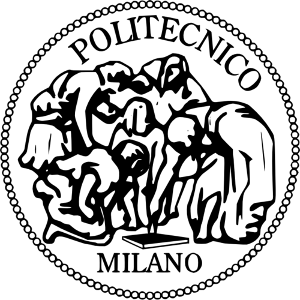
\includegraphics[width=0.5\textwidth]{img/logo.png}}


\author{Alessio Russo, Gianluca Savaia, Alberto Ficicchia}
\title{Control of Linear Vibrations \\
\Large Automation and Control Laboratory \\
 Politecnico di Milano}
\date{Academic Year 2015/2016}








\begin{document}
\maketitle
\tableofcontents

\clearpage
\subimport*{parts/Team/}{main.tex}
\newpage
\subimport*{parts/Experience/}{main.tex}
\newpage
\subimport*{parts/Models/}{main.tex}
\newpage
\subimport*{parts/Identification/}{main.tex}
\newpage
\part{System control}
\subimport*{parts/Control1dof/}	{main.tex}
\newpage
\subimport*{parts/Control2dof/}{main.tex}
\newpage
\subimport*{parts/Control3dof/}{main.tex}
\newpage
\subimport*{parts/Conclusions/}{main.tex}
\newpage
\subimport*{parts/Appendix/}{main.tex}

\addcontentsline{toc}{chapter}{Bibliography}
\printbibliography

\end{document}